\documentclass[fontset=windows]{article}
\usepackage[margin=1in]{geometry}
\usepackage{ctex}
\usepackage{setspace}
\usepackage{lipsum}
\usepackage{graphicx}
\usepackage{caption}
\usepackage{subcaption}
\usepackage[colorlinks=true,linkcolor=red]{hyperref}

\graphicspath{{figures/}}

\title{\heiti\zihao{2} Introduction to MOSFETs}
\author{\songti zrrraa}
\date{2023.11.12}

\begin{document}
\maketitle
\thispagestyle{empty}

\section*{How the MOSFET Come}
\begin{figure}[htbp]
    \centering
    \rotatebox{90}{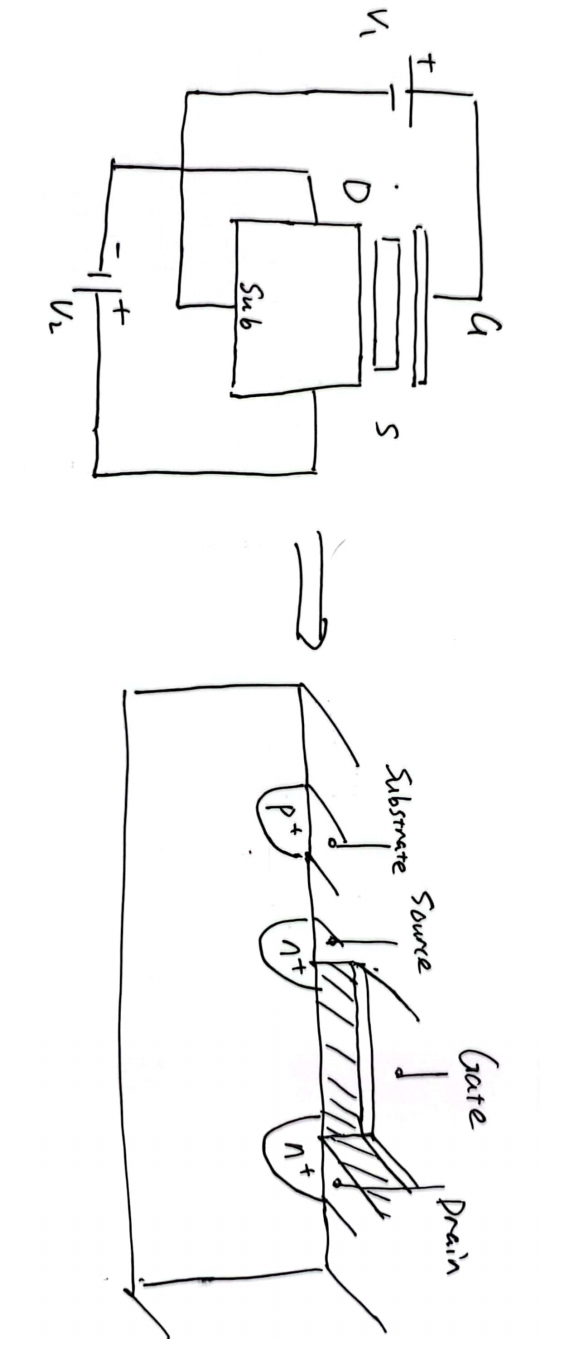
\includegraphics[scale=0.6]{1.jpg}}
    \captionsetup{labelformat=empty}
    \caption{The origin of the three-dimensional diagram of the MOSFET}
    \label{1}
\end{figure}

When $V_1$ is added to both ends of a capacitor, electrons accumulate on the lower plate;
after $V_2$ is added to both ends of the lower plate, the electrons start to move under the action of the electric field, forming a current.
This is the simplest MOSFET model. We cannot operate the side of the wafer, so we extend the two ends of the lower plate to the front.
Then it comes to a three-dimensional diagram of the MOSFET.

\

The full name of MOSFET is Metal Oxide Semiconductor Field Effect Transistor.
Metal refers to the electrode of the gate, with an insulating layer of silicon dioxide underneath.

Therefore, the current flowing from the gate can be almost ignored.

The smaller the thickness of the insulating layer, the larger the capacitance, the more electrons are attracted, and the larger $I_D$ is.

\

Flip the model, we get the circuit symbol of MOSFET.

\begin{figure}[htbp]
    \centering
    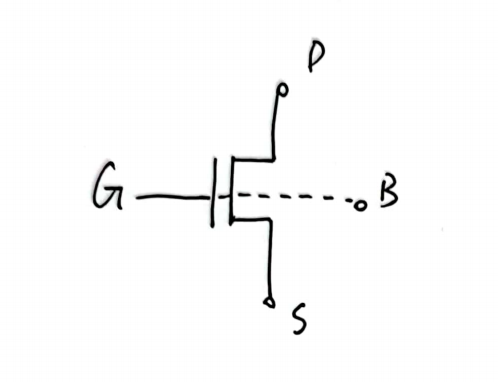
\includegraphics[scale=0.6]{2.jpg}
    \captionsetup{labelformat=empty}
    \caption{Circuit symbol of MOSFET}
    \label{2}
\end{figure}

The Source and the Drain are symmetrical. We can't tell which is which. The Substrate can be anywhere.

The level of the Substrate (or Bulk) is usually given, so its symbol is generally not marked

\section*{MOS Operation}

$V_{th}$: The voltage at which we introduce electrons instead of the negative ions.

Depletion: Deplete the holes.

\

Now let us start to learn some operation about MOSFET.

\subsection*{$V_D=V_S=0$}

We begin at applying voltage to the Gate and connect the Source and the Drain to the ground.

\begin{figure}[htbp]
    \centering
    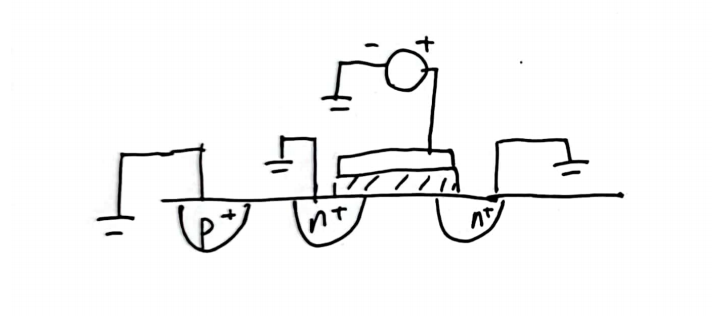
\includegraphics[scale=0.6]{3.jpg}
    \captionsetup{labelformat=empty}
    \caption{Apply voltage to the Gate}
    \label{3}
\end{figure}

When the $V_G$ increase, the attraction of the Gate increase.

When the $V_G=V_{th}$, A channel appears between two n-type semiconductors and begins to conduct electricity.

When the $V_G>V_{th}$, the MOSFET becomes a voltage controlled resistor.

\begin{figure}[htbp]
    \centering
    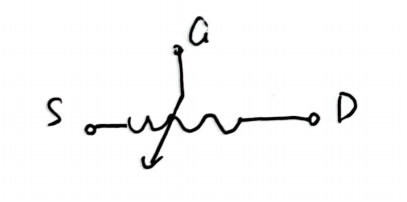
\includegraphics[scale=0.6]{4.jpg}
    \captionsetup{labelformat=empty}
    \caption{Voltage controlled resistor}
    \label{4}
\end{figure}

\subsection*{$V_D>V_S=0$}

Then we add voltage to the Drain.

\begin{figure}[htbp]
    \centering
    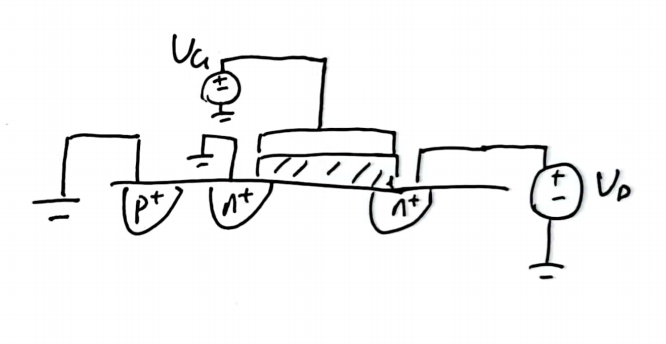
\includegraphics[scale=0.6]{5.jpg}
    \captionsetup{labelformat=empty}
    \caption{Apply voltage to the Gate and the Drain}
    \label{5}
\end{figure}

The control variable method is very commonly used in Teacher Razavi's class.
We consider $V_D=constant$ first.

\begin{figure}[ht]
    \centering
    \begin{subfigure}[b]{0.3\textwidth}
        \centering
        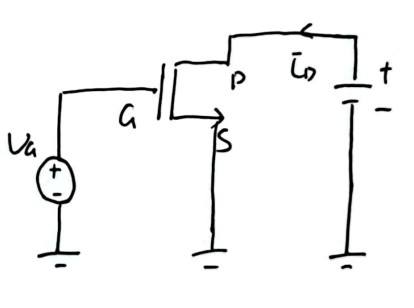
\includegraphics[width=\textwidth]{6.jpg}
        \label{fig:subfig1}
    \end{subfigure}
    \hfill
    \begin{subfigure}[b]{0.45\textwidth}
        \centering
        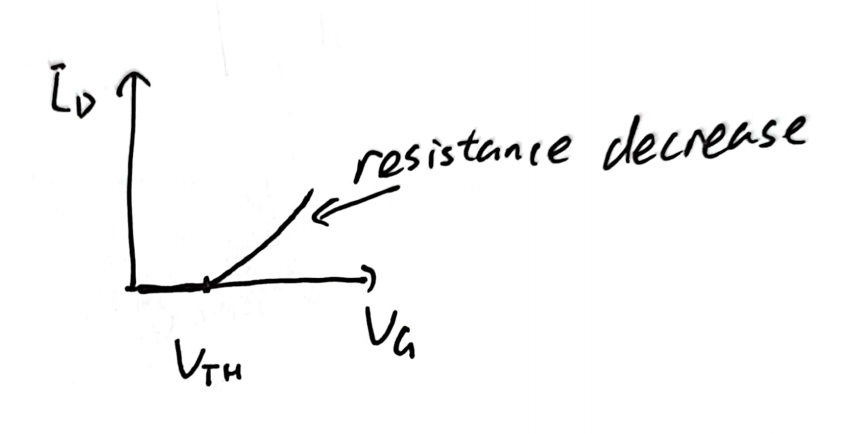
\includegraphics[width=\textwidth]{7.jpg}
        \label{fig:subfig2}
    \end{subfigure}
    \captionsetup{labelformat=empty}
    \caption{$V_D=constant, \ e.g. 0.3V$}
    \label{fig:both1}
\end{figure}

Then we consider $V_G=constant$.

\begin{figure}[ht]
    \centering
    \begin{subfigure}[b]{0.3\textwidth}
        \centering
        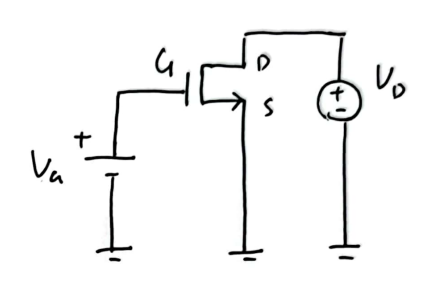
\includegraphics[width=\textwidth]{8.jpg}
        \label{fig:subfig3}
    \end{subfigure}
    \hfill
    \begin{subfigure}[b]{0.45\textwidth}
        \centering
        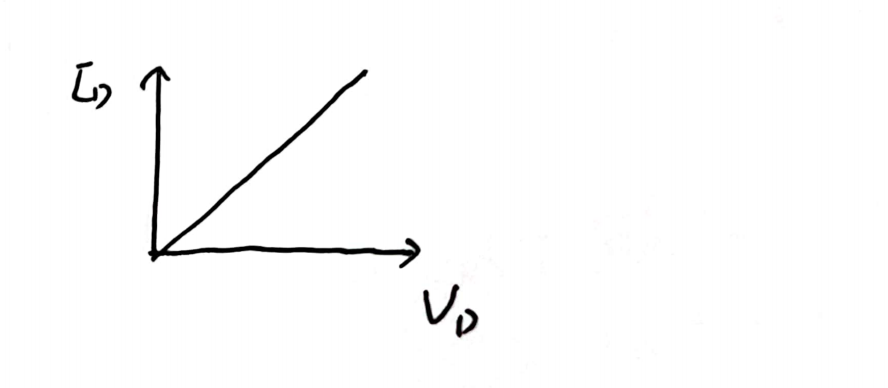
\includegraphics[width=\textwidth]{9.jpg}
        \label{fig:subfig4}
    \end{subfigure}
    \captionsetup{labelformat=empty}
    \caption{$V_D=constant, \ e.g. 1V$}
    \label{fig:both2}
\end{figure}

These are the simplest models, next we will learn more accurate models.

\section*{Link}

\href{https://www.bilibili.com/video/BV1FD4y1R7Ah?p=29&vd_source=1d0c07486a3bd3b0adb8ac548bf6453e}{Razavi Electronics Circuits 1: lectrue 29}
\end{document}